\section{Continuous Integration/Delivery}
\subsection{GitHub Actions}

allg. actions warum kosten
\subsubsection{Build IOS}
\author{Martin Hausleitner}

\subsubsection{Build Android}

\subsection{Fastline}
\subsubsection{Build Number increment}
\subsection{Firebase App Distribution}

\section{Mobile Anwendung}
\subsection{Dateistruktur}
\author{Martin Hausleitner}
In Flutter gibt es keine fixe Dateistruktur für eine App,
man kann seine Struktur also selbst überlegen und gestalten.
Im Folgenden beschreibe ich, wie wir unsere Dateistruktur
für eine Flutter-App aufgebaut haben.

In Flutter gibt es keine feste Dateistruktur, stattdessen kann man die Struktur der Dateien und Ordner selbst bestimmen. Für unser Flutter-Projekt haben wir uns für eine Struktur entschieden, die sich an bewährten Praktiken orientiert.

Unsere Dateistruktur sieht wie folgt aus:

\begin{itemize}
    \item \textbf{logic} - Hier befindet sich die Geschäftslogik der App, einschließlich der Firestore-Cloud-Funktionen und Repositories, die API-Aufrufe ausführen.
    \item \textbf{pages} - Hier werden Widgets entworfen, die jeweils eine Seite der App darstellen.
    \item \textbf{routes} - Hier werden die Routen definiert, die tiefere Links ermöglichen.
    \item \textbf{shared} - Hier werden UI-Widgets wie Buttons oder andere Widgets gespeichert, die oft wiederverwendet werden.
    \item \textbf{views} - Hier befinden sich Ansichten, die von mehreren Seiten der App verwendet werden können.
\end{itemize}

Im Nachhinein hätten wir die Dateistruktur anders gestaltet,
z.B. hätten wir das UI als eigenes Package definiert und die
pages und views besser unterteilt.

\subsection{State Management}
In Flutter gibt es verschiedene Möglichkeiten\cite{flutter-docs-interactive}\cite{flutter-state-management-blog}, um mit dem State Management umzugehen. State Management bezieht sich auf die Art und Weise, wie Daten innerhalb einer App verwaltet werden. In jeder App gibt es bestimmte Daten, die von verschiedenen Komponenten und Widgets verwendet werden und sich im Laufe der Zeit ändern können. State Management bezieht sich auf die Methoden, die verwendet werden, um diese Daten innerhalb der App zu verwalten und zu aktualisieren.
\author{Martin Hausleitner}

\subsubsection{GetX}
\author{Martin Hausleitner}

GetX verwendet ein reaktives Ansatz zur Verwaltung des Zustands, was bedeutet, dass Änderungen im Zustand automatisch die UI aktualisieren, ohne dass der Entwickler manuell Code schreiben muss, um diese Aktualisierungen durchzuführen. Dies spart viel Entwicklungszeit und macht es einfach, auf Benutzerinteraktionen zu reagieren.

Mit GetX können wir auch eine einheitliche Datenquelle haben, auf die alle Komponenten zugreifen können, was die Wartung und Erweiterung der Anwendung erleichtert. Darüber hinaus bietet GetX auch eine einfache Möglichkeit, Abhängigkeiten zu verwalten und Zustandsinformationen zwischen Bildschirmen zu teilen.

Insgesamt hat uns die Verwendung von GetX im Flutter-Framework sehr geholfen, eine effektive und skalierbare Anwendung zu erstellen, die auf die Bedürfnisse unserer Benutzer abgestimmt ist.
\author{Sandin Habibovic}
getx controller service etc...


\subsection{Authentifizierung}
\author{Sandin Habibovic}

\subsubsection{Anmelde Flow}
\author{Sandin Habibovic}

Diagram
erklärung
screenshots
\subsubsection{Regestrierungs Flow}
\author{Sandin Habibovic}


Diagram
erklärung
screenshots


\subsubsection{Firebase Authentifizierung}
\author{Sandin Habibovic}

allg.


\subsection{Feed}
\author{Sandin Habibovic}
foto
aufbau

\subsection{Beiträge}
\author{Sandin Habibovic}
Beiträge sind das Hauptkommunikationsmittel auf der App. Jedem Beitrag muss ein Titel, eine Beschreibung und eine Reichweite, unter der, der Beitrag sichtbar ist, angegeben werden. Weiters ist es möglich einem Beitrag ein Bild und Tags anzuhängen.

\subsubsection{Kategorien}
\author{Sandin Habibovic}
Um Beiträge besser zuordnen zu können, muss der User den Beitrag vor dem Veröffentlichen in eine bestimmte Kategorie einteilen. Diese Kategorien ermöglichen es Usern, die Art Ihrer Anfrage ihm vorhinein besser zu spezifizieren und die Suche nach Beiträgen einer bestimmten Art zu vereinfachen. Bestimmte Kategorien werden weiters in Unterkategorien aufgeteilt, da diese ein zu weit gefächertes Genre an Anfragen umfassen.

Es existieren folgende Kategorien bzw. Unterkategorien:

\begin{compactitem}
    \item Mitteilung
    \begin{compactitem}
        \item Frage
        \item Appell
        \item Warnung
        \item Empfehlung
        \item Gefunden
    \end{compactitem}
    \item Suche
    \begin{compactitem}
        \item Hilfe
        \item Verloren
    \end{compactitem}
    \item Ausleihen
    \item Event
\end{compactitem}



Mitteilung:
Die Kategorie der Mitteilung dient dazu die Nachbarn über ein bestimmtes Ereignis oder Meldung zu informieren oder zu befragen.

Suche:
Die Kategorie der Suche dient dazu mit den Nachbarn im Falle einer Hilfesuche oder eines verloren gegangenen Objekts in Kontakt zu treten.

Ausleihen:
Die Kategorie des Ausleihens dient dazu die Nachbarn nach der Erlaubnis, sich ein bestimmtes Werkzeug oder Objekt ausborgen zu dürfen, zu bitten.

Event:
Die Kategorie des Events dient dazu die Nachbarn auf eine bestimmte Veranstaltung aufmerksam zu machen.


\subsubsection{Tags}
\author{Sandin Habibovic}
Als Tag wird ein Schlüsselwort beschrieben, was man an ein Informationsgut anhängen kann, um es besser beschreiben zu können und/oder besser auffindbar zu machen. In der App werden Tags als eine Erweiterung der Kategorien verwendet, um es Usern zu ermöglichen Ihren Beitrag einem selbstdefinierten Typ zuzuordnen.

\subsubsection{Info}
\author{Sandin Habibovic}
Jeder Beitrag hat eine eigene Sektion, wo wichtige Entscheidungsinformationen angegeben werden, wie der Stadtteil und die ungefähre Entfernung zum gegebenen Nachbarn und das Erstelldatum des Beitrags.

\subsubsection{Kommentare}
\author{Sandin Habibovic}
Die Kommentarfunktion ermöglicht es den Usern unter einem Beitrag Ihre Meinung, Feedback oder sonstiges zu hinterlassen.

\subsubsection{Beitrag oder Kommentar Melden}
\author{Sandin Habibovic}
Um auf unangebrachte Beiträge oder Kommentare schnell reagieren zu können, gibt es die Möglichkeit Beiträge oder Kommentare zu melden. Diese Meldungen werden auf Firestore gespeichert und können dann im Einzelnen überprüft werden. Fürs Melden muss ein Grund ausgewählt und eine genauere Beschreibung angegeben werden.
Gründe fürs Melden eines Beitrags oder Kommentars:

\begin{compactitem}
    \item Unangebrachter Inhalt
    \item Belästigung
    \item Betrug
    \item Spam
    \item Sonstiges
\end{compactitem}

\subsection{Filter}
\author{Sandin Habibovic}
Filtern nach Kategorien
Ordnen nach Likes oder Datum
Absteigend oder aufsteigend sortieren

\subsection{Suche}
\subsection{Typesense}
\subsection{Algolia}
diagram
\subsubsection{Firestore Sync}

\subsubsection{Algolia SDK}


\subsection{Chat}
package genommen warum
\subsubsection{Flyer Package}

\subsection{Profil}
\author{Sandin Habibovic}
Was wird angezeigt?
Name, User Public Info, Posts von User

\subsubsection{Profil Melden}
\author{Sandin Habibovic}

\subsection{Benachrichtigungen}
\author{Sandin Habibovic}
Grund und Funktionsweise von Benachrichtigungen
diagram beschreibung
\subsection{Einstellungen}
\author{Sandin Habibovic}
Email/Passwort ändern, Konto löschen, Sprache einstellen, Benachrichtigungen ein/ausschalten
\subsection{Feedback}
\author{Martin Hausleitner}
feedback feature beschreiben


\section{UI/UX Design}
Das UI/UX-Design einer App ist von entscheidender Bedeutung für den Erfolg der App und die Zufriedenheit der Benutzer. Insbesondere bei einer Social-Media-Nachbarschafts-App ist ein gut durchdachtes UI/UX-Design unerlässlich, um eine positive Benutzererfahrung zu gewährleisten.

Ein gutes UI-Design ist wichtig, um sicherzustellen, dass die Benutzer die App einfach und intuitiv bedienen können. Es sollte eine klare Struktur und Navigation haben, damit die Benutzer schnell zu den gewünschten Funktionen gelangen können. Wenn die Benutzer die App als kompliziert oder verwirrend empfinden, werden sie möglicherweise frustriert und geben die Nutzung der App auf.

Auch ein gutes UX-Design ist wichtig, um sicherzustellen, dass die Benutzer mit der App zufrieden sind. Es sollte eine ansprechende und ansprechende Benutzeroberfläche bieten, die dem Benutzer ein angenehmes Nutzungserlebnis vermittelt. Wenn die Benutzer die App als langweilig oder uninteressant empfinden, werden sie möglicherweise nicht wiederkommen.

Darüber hinaus sollte das UI/UX-Design einer Social-Media-Nachbarschafts-App bestimmte Funktionen und Merkmale berücksichtigen, die für eine erfolgreiche Community-Plattform erforderlich sind. Beispielsweise sollte es einfach sein, Beiträge zu erstellen und zu teilen, auf Kommentare zu antworten und Nachrichten an andere Benutzer zu senden. Es sollte auch Möglichkeiten geben, um Benutzerprofile zu erstellen und zu verwalten sowie umfassende Datenschutz- und Sicherheitsfunktionen zu bieten.

Insgesamt ist das UI/UX-Design einer Social-Media-Nachbarschafts-App von entscheidender Bedeutung für den Erfolg der App und die Zufriedenheit der Benutzer. Es ist wichtig, dass das Design auf die Bedürfnisse und Anforderungen der Benutzer zugeschnitten ist und ein einfaches, intuitives und ansprechendes Nutzungserlebnis bietet.
\author{Martin Hausleitner}
\subsection{Inspiration}
Während des Designprozesses für die App habe ich umfangreiche Recherchen im Bereich App-Design durchgeführt. Mein Ziel war es, die App so intuitiv wie möglich zu gestalten, um eine benutzerfreundliche Erfahrung zu gewährleisten. Dazu habe ich mich an bekannten Social-Media-Apps orientiert, wie zum Beispiel Twitter, Instagram und TikTok, die bereits auf dem Markt sehr erfolgreich sind und von vielen Menschen vertraut genutzt werden.

Darüber hinaus hat auch die erfolgreichste Nachbarschafts-App in Deutschland, "Nebenan", viel zur Grundlage der App beigetragen. Allerdings habe ich festgestellt, dass ihre App sehr kompliziert aufgebaut und unübersichtlich ist, was für uns eine Chance darstellte, es besser zu machen.

Zusätzlich haben wir uns von Websites wie Dribble und Mobbin inspirieren lassen, die uns geholfen haben, ein einfaches und schlichtes Design für die App zu entwickeln. Insgesamt war die Recherche und Inspiration für das Design der App ein wichtiger Schritt, um sicherzustellen, dass unsere Benutzer eine ansprechende und intuitive Erfahrung haben.

\subsection{Prototyping}
Prototyping ist ein wichtiger Schritt bei der Entwicklung von mobilen Apps. Es ermöglicht Entwicklern, Designern und anderen Stakeholdern, eine frühzeitige Vorstellung davon zu bekommen, wie die App funktionieren wird und wie sie aussehen wird. Durch die Erstellung eines Prototyps können auch Fehler im Design und in der Funktionalität identifiziert werden, bevor die App in die eigentliche Entwicklung geht.

Es gibt verschiedene Arten von Prototypen, darunter Low-Fidelity- und High-Fidelity-Prototypen. Low-Fidelity-Prototypen sind einfache Skizzen oder Wireframes, die nur die grundlegenden Funktionen und das Layout der App abbilden. High-Fidelity-Prototypen sind detaillierter und können interaktive Funktionen und Designelemente enthalten.

Es gibt viele Tools und Plattformen, die zur Erstellung von Prototypen verwendet werden können. Ein Beispiel ist Adobe XD, das es Entwicklern und Designern ermöglicht, schnelle und einfache Prototypen zu erstellen. Andere Tools wie Sketch, Figma oder InVision sind ebenfalls beliebt.

Der Vorteil von Prototyping ist, dass es Entwicklern und Designern ermöglicht, frühzeitig Feedback von Benutzern zu erhalten und Änderungen vorzunehmen, bevor die App tatsächlich entwickelt wird. Außerdem können Entwickler und Designer Zeit und Ressourcen sparen, indem sie sich auf die richtigen Funktionen und das richtige Design konzentrieren und unnötige Funktionen und Designs vermeiden.

Im Fall von Flutter als Entwicklungsplattform für die App ist das Prototyping ebenfalls wichtig. Flutter bietet verschiedene Widgets und Design-Tools, mit denen Entwickler schnell und einfach Designelemente erstellen und implementieren können. Durch ein gut durchdachtes Prototyping kann Zeit und Aufwand beim Entwickeln gespart werden, da Design-Entscheidungen bereits getroffen wurden und Entwickler sich auf die Umsetzung konzentrieren können.

Insgesamt ist Prototyping ein unverzichtbarer Schritt bei der Entwicklung von mobilen Apps. Es ermöglicht Entwicklern und Designern, frühzeitig Feedback von Benutzern zu erhalten und Änderungen vorzunehmen, bevor die App tatsächlich entwickelt wird. Durch die Verwendung von Tools wie Adobe XD, Sketch oder Figma können Prototypen schnell und einfach erstellt werden, was Zeit und Ressourcen spart. Prototyping ist auch für die Verwendung von Flutter als Entwicklungsplattform wichtig, da es Entwicklern ermöglicht, Zeit und Aufwand zu sparen und sich auf die Umsetzung zu konzentrieren.
\subsubsection{Framer}
Framer ist eine Software, die es Benutzern ermöglicht, schnell und einfach ansprechende Prototypen von mobilen Anwendungen und Websites zu erstellen. Das Tool wurde ursprünglich als Prototyping-Tool für Designer entwickelt, um Designs schnell zu testen und zu verfeinern, bevor sie in die Entwicklung übergehen.

Erfolgreiche Apps wie Spotify haben Framer im Rahmen ihres Prototyping-Prozesses verwendet, um schnell und effizient funktionierende App-Designs zu erstellen. Framer ist eine schnelle und effiziente Möglichkeit, um Ideen in die Tat umzusetzen, ohne sich durch langwierige Entwicklungsprozesse zu quälen.

Framer wurde während des Hackerthon Linz hackt verwendet, um den ersten Prototypen zu erstellen. Die Wahl von Framer war aufgrund seiner Geschwindigkeit und Effizienz in der Erstellung von funktionsfähigen App-Designs und der Erfahrung, die der Benutzer bereits mit dem Tool hatte, getroffen worden.

Seit der Erstellung des ersten Prototyps hat sich das Geschäftsmodell von Framer jedoch geändert. Es ist jetzt ein Website-Baukasten, der es Benutzern ermöglicht, einfach und schnell ansprechende Websites zu erstellen, ohne Kenntnisse in der Webentwicklung zu benötigen. Obwohl es nun als Website-Baukasten fungiert, behält Framer immer noch einige seiner Kernfunktionen als Prototyping-Tool bei, was es zu einer guten Option für Designer und Entwickler macht, die schnell Prototypen erstellen möchten.

Insgesamt hat Framer gezeigt, dass es ein schnelles und effektives Tool ist, um Designideen in die Tat umzusetzen. Obwohl es nun als Website-Baukasten fungiert, ist es immer noch eine nützliche Option für Designer und Entwickler, die schnell und einfach Prototypen erstellen möchten.

\subsubsection{Adobe XD}
Als ich zum ersten Mal mit Framer arbeitete, war ich begeistert von den vielen Features und Möglichkeiten, die es bietet. Aber im Laufe der Zeit stellte ich fest, dass es für mein Projekt zu aufwändig war und ich nach einer einfacheren Lösung suchte. So bin ich auf Adobe XD umgestiegen, ein Tool, mit dem ich schon jahrelange Erfahrung hatte.

Obwohl Adobe XD nicht so viele Features wie Framer bietet,
ist es aufgrund seiner Einfachheit und
Benutzerfreundlichkeit ein ideales Tool, um schnell einen
Prototypen zu erstellen. Ich hatte alle Hauptscreens
fertig gestaltet, bevor wir mit der Entwicklung mit Flutter
begannen. Die anderen wichtigen Screens habe ich dann
später gestaltet, als ich mit Flutter vertrauter war und
besser abschätzen konnte, wie aufwändig es in Flutter
umzusetzen war.

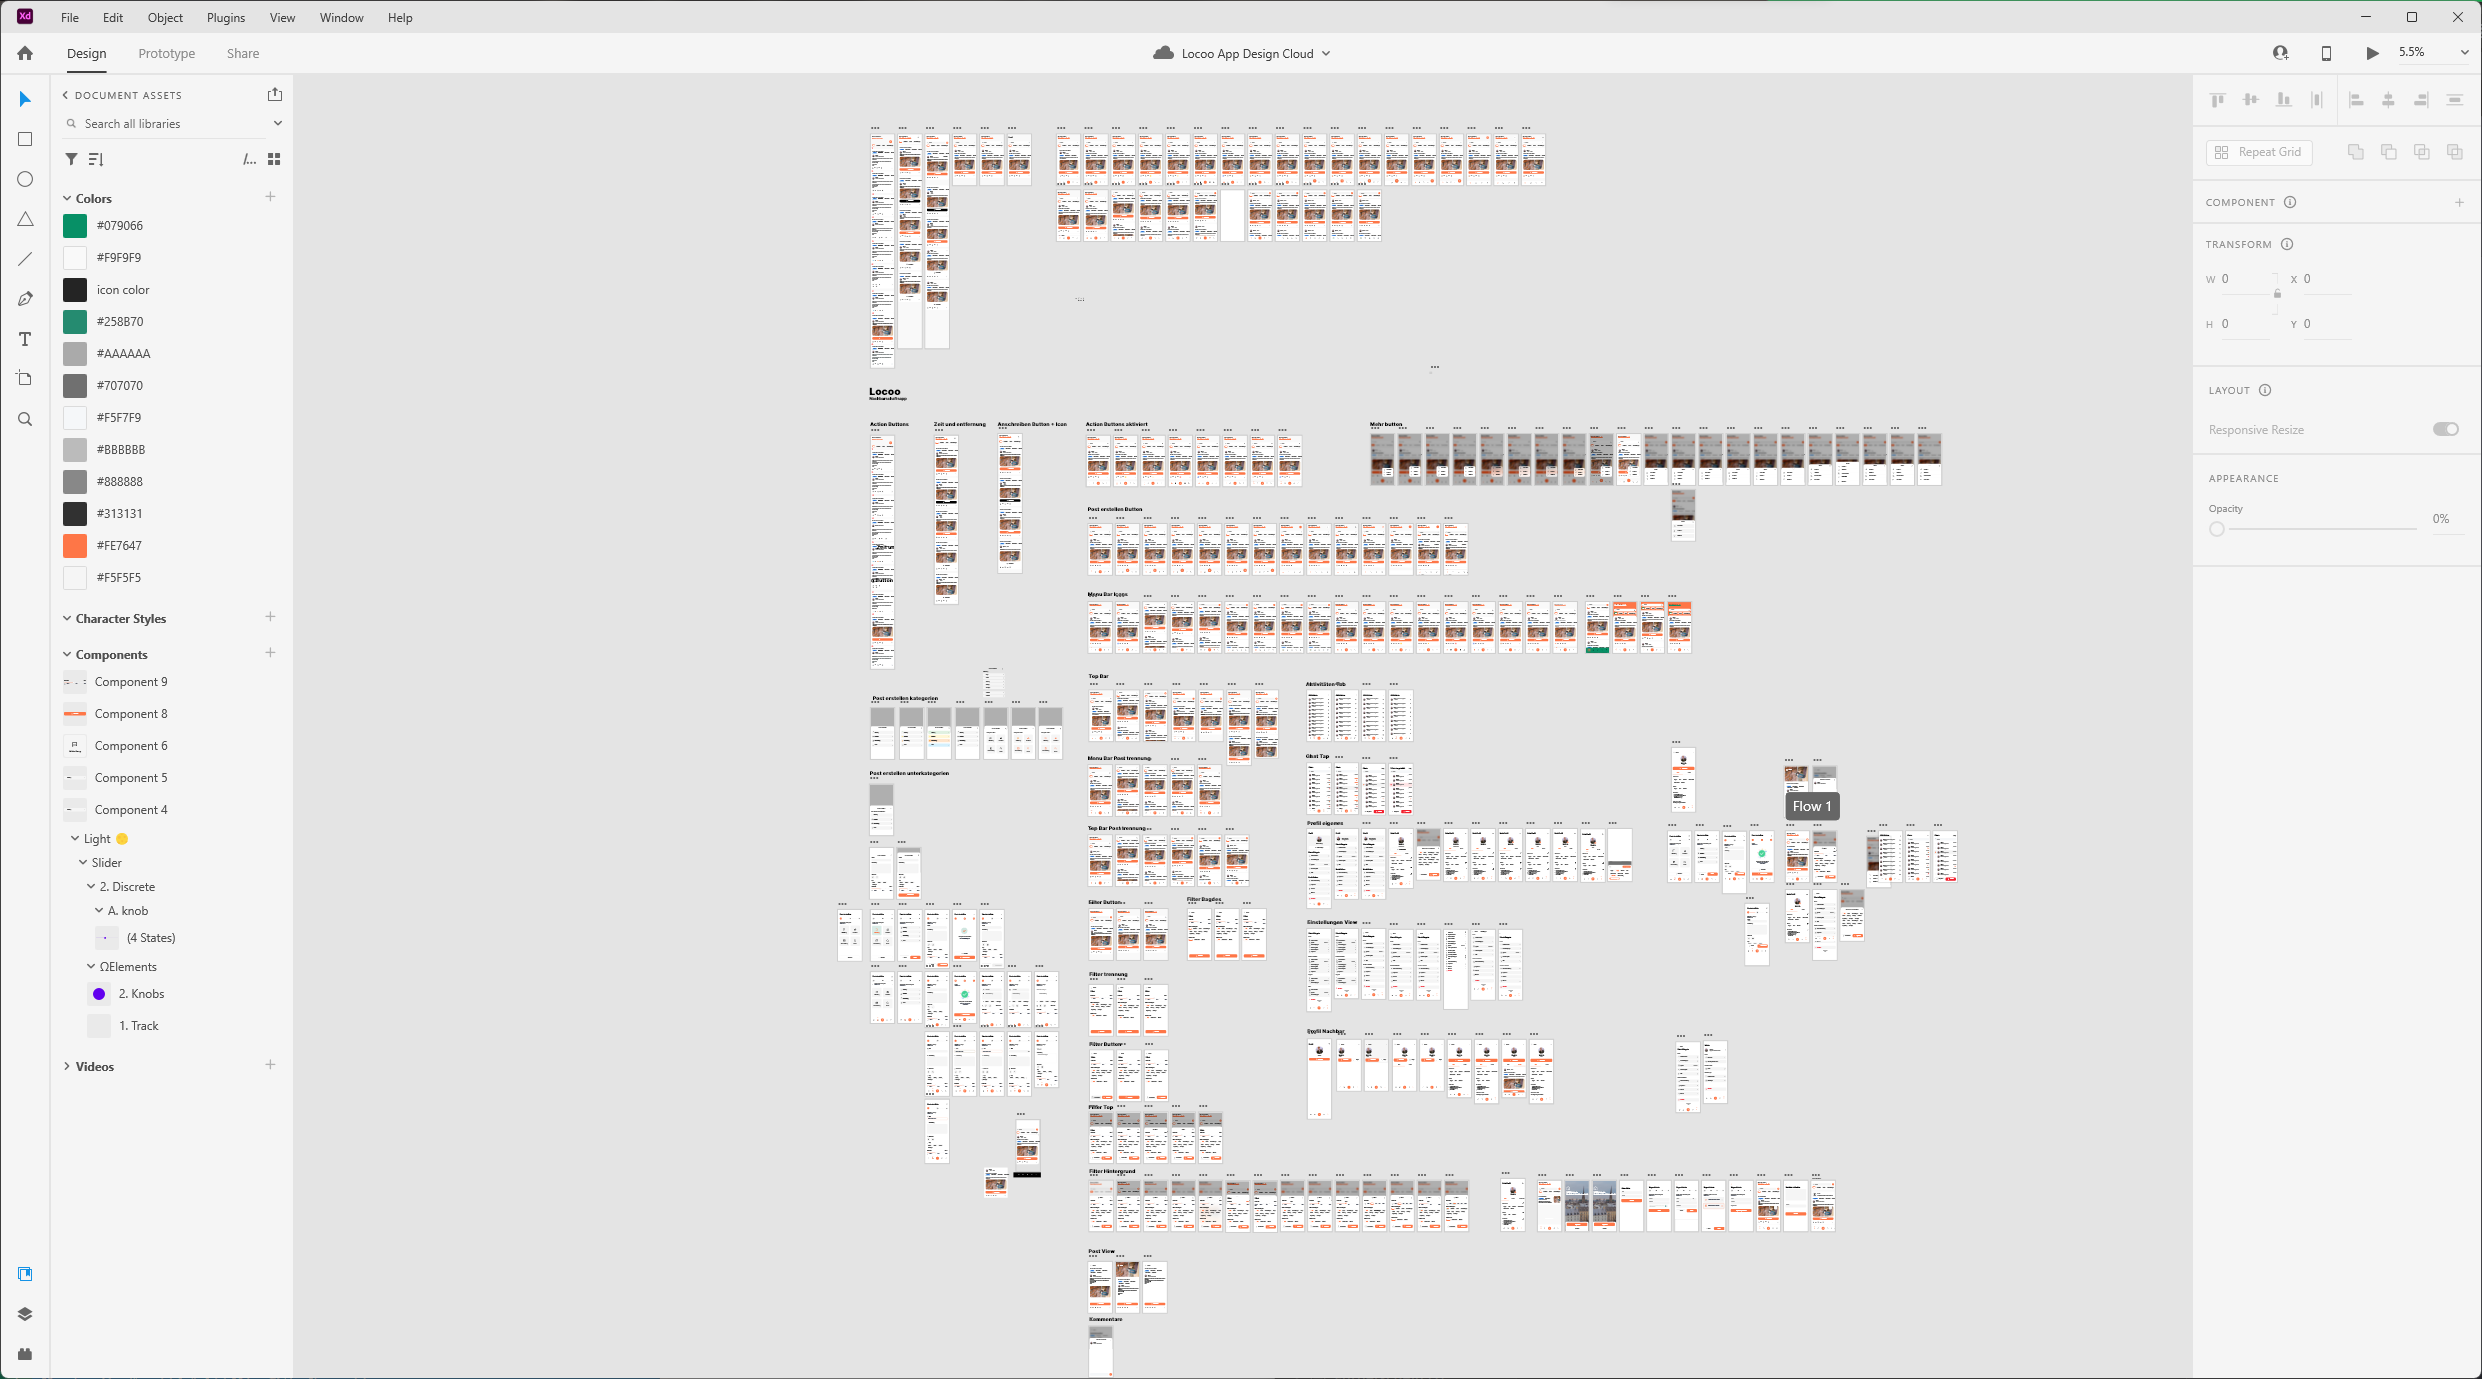
\includegraphics[width=0.95\textwidth]{pics/nochba-adobe-xd-protoype-screenshot.png}


Wie man auf dem obigen Bild sehen kann, ist unser Prototyp
eine Sammlung verschiedener Designs und Evolutionen des
Designs. Adobe XD war für unser Projekt perfekt, da ich der
alleinige Designer war und somit keine
Kollaborationsfunktion benötigte. Allerdings, da ich jetzt
mit dem bekanntesten Designtool Figma vertraut bin und es billiger ist, wenn mehrere
Personen an einem Design arbeiten und auch mehr Funktionen
bietet, würde ich aktuell mit Figma weiterarbeiten.

Zusammenfassend lässt sich sagen, dass Adobe XD ein mächtiges Tool für UI/UX-Designer ist, das einfach zu bedienen und ideal für kleine bis mittelgroße Projekte ist. Es bietet zwar nicht so viele Funktionen wie andere Tools, ist aber für schnelle Prototypenerstellung und einfache Zusammenarbeit mit Entwicklern und Stakeholdern sehr gut geeignet.

\subsection{Design}
design patterns
\subsubsection{Farben}
farben history
warum orange
\subsubsection{Icons}
foto von den benutzen icons
welche icons
warum
\subsubsection{Fonts}
fotos von fonts
welche fonts
wie ist due typrographie aufgebaut
\subsubsection{Logo}
logo foto
anforderungen
design ideen
logo history
\subsection{App Design}
eingehen mit fotos und beschreibung auf die haupt screens der app

\subsection{Websiten Design}
2-3 nochba.at design foto
beschreibung

\section{Backend}
\subsection{Cloud}
\author{Martin Hausleitner}

\subsection{Firebase}
\author{Martin Hausleitner}

\subsubsection{Firebase SDKs}
\author{Sandin Habibovic}
Firebase-Tools

\subsubsection{Firebase Authentication}
\author{Sandin Habibovic}
Email und Passwort authentication

\subsubsection{Cloud Firestore}
\author{Sandin Habibovic}
NoSQL-Database, Dokument-basierte Speicherung, Subcollections
\subsubsection{Cloud Storage}
\author{Sandin Habibovic}
Speicherung von Profilbilder und Post-Bilder
\subsubsection{Firebase Cloud Functions}
jeder schreibt über seine CF

\subsection{Algolia Search}
\subsection{Algolia SDK}

\subsubsection{Typesense Search}
\subsection{Typesense SDK}
